\chapter{Controle Bancário: Versão 4}\label{interface}

Neste  capítulo,   dando  continuidade   ao  desenvolvimento  em   Grails,  será
apresentado o  processo de  desenvolvimento da quarta  versão da  aplicação {\bf
  ControleBancario}. Nessa versão são incorporadas as seguintes funcionalidades:

\begin{itemize}

\vspace{0.5cm}

\item Implementação  da funcionalidade de  visualização e impressão  de extratos
  bancários associados às  contas bancárias. Para tal, serão  utilizados os {\it
    plugins} {\bf wkhtmltopdf} e {\bf google-visualization};

\vspace{0.5cm}

\item  Implementação de  um serviço  {\it web}  REST que  retorna uma  lista (em
  formato JSON ou XML) de agências de um determinado banco; 

\end{itemize}

\section{Configuração da aplicação} 

\vspace{0.5cm}

\noindent{\bf   Instalação   de    {\it   plugins}.}    Na   implementação   das
funcionalidades da aplicação  {\bf ControleBancario}, discutidas nesse capítulo,
serão  utilizados os  {\it plugins}  Grails {\bf  richui}, {\bf  pure-css}, {\bf
  wkhtmltopdf} e  {\bf google-visualization}. Conforme  discutido anteriormente,
para  instalar   esses  {\it  plugins},  adicione  as   linhas,  descrevendo  as
dependências,  no  arquivo  {\bf  BuildConfig.groovy} conforme  apresentado  nas
linhas 54-57 do Código~\ref{codBuildConfig4}.  
\index{Plugins!richui}
\index{Plugins!pure-css}
\index{Plugins!wkhtmltopdf}
\index{Plugins!google-visualization}

\newpage

\begin{lstlisting}[numbers=left,  caption={\bf  BuildConfig.groovy}, frame=trBL,
    float=htbp, label=codBuildConfig4]
grails.project.dependency.resolution = {
    // inherit Grails' default dependencies
    inherits("global") {
        // specify dependency exclusions here; for example, uncomment this to disable ehcache:
        // excludes 'ehcache'
    }
    log "error" // log level of Ivy resolver, either 'error', 'warn', 'info', 'debug' or 'verbose'
    checksums true // Whether to verify checksums on resolve
    legacyResolve false // whether to do a secondary resolve on plugin installation, not advised and 
                        // here for backwards compatibility

    repositories {
        inherits true // Whether to inherit repository definitions from plugins

        grailsPlugins()
        grailsHome()
        mavenLocal()
        grailsCentral()
        mavenCentral()
        // uncomment these (or add new ones) to enable remote dependency resolution from public Maven repositories
        mavenRepo "http://repository.codehaus.org"
        //mavenRepo "http://download.java.net/maven/2/"
        //mavenRepo "http://repository.jboss.com/maven2/"
        mavenRepo "http://repo.spring.io/milestone/"
    }

    dependencies {
        // specify dependencies here under either 'build', 'compile', 'runtime', 'test' or 'provided' scopes e.g.
        // runtime 'mysql:mysql-connector-java:5.1.27'
        runtime 'org.postgresql:postgresql:9.3-1100-jdbc41'
    }

    plugins {
        // plugins for the build system only
        build ":tomcat:7.0.50"

        // plugins for the compile step
        compile ":scaffolding:2.0.1"
        compile ':cache:1.1.1'

        // plugins needed at runtime but not for compilation
        runtime ":hibernate:3.6.10.7" // or ":hibernate4:4.1.11.6"
        runtime ":database-migration:1.3.8"
        runtime ":jquery:1.10.2.2"
        runtime ":resources:1.2.1"
        // Uncomment these (or add new ones) to enable additional resources capabilities
        //runtime ":zipped-resources:1.0.1"
        //runtime ":cached-resources:1.1"
        //runtime ":yui-minify-resources:0.1.5"
        
        compile ":br-validation:0.3"
        compile ":spring-security-core:2.0-RC2"
        compile ":rest:0.8"
        compile ":richui:0.8"
        compile ":pure-css:0.4.2"
        compile ":wkhtmltopdf:0.1.7"
        compile ":google-visualization:0.7"
    }
}
\end{lstlisting}

\noindent{\bf Instalação  do wkhtmltopdf.} Na versão,  discutida nesse capítulo,
extratos bancários, associados às contas bancárias, poderão ser convertidos para
o formato pdf.  Para tal, será necessária a instalação do {\bf wkhtmltopdf}, que
consiste em uma ferramenta {\it open-source} que converte arquivos {\bf html} em
arquivos {\bf pdf}. 

A instalação no  sistema operacional linux Ubuntu pode  ser realizada através do
comando  {\bf sudo  apt-get  install wkhtmltopdf  -q},  conforme apresentada  na
Figura~\ref{figWkhtmltopdf}.  

\vspace{0.5cm}

\begin{remark}
Para  os demais  sistemas operacionais,  sugere-se  ao leitor  que verifique  as
instruções           de           instalação           disponíveis           em:
{\footnotesize\url{http://wkhtmltopdf.org}}.  
\end{remark}

\begin{figure}[htbp]
\centering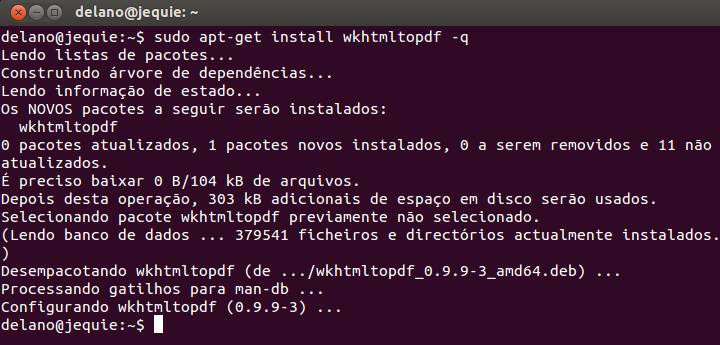
\includegraphics[width=12cm]{wkhtmltopdf}
\caption{Instalação do {\bf wkhtmltopdf}}
\label{figWkhtmltopdf}
\end{figure}

\newpage

\noindent{\bf  Configuração  de {\it  plugins}.}   Após  a  instalação dos  {\it
  plugins}  é   necessário  incluir   algumas  configurações  no   arquivo  {\bf
  conf/Config.groovy} (Código~\ref{codConfig}). Por questão de brevidade, apenas
serão apresentadas as mudanças realizadas nesse arquivo.  

\begin{itemize}

\vspace{0.3cm}

\item O primeiro bloco adiciona o  formato {\bf pdf} na lista de {\it MimeTypes}
  manipulados pela aplicação;

\vspace{0.3cm}

\item O segundo bloco configura a maneira em que os {\it scriptlets} (trechos de
  código)  são tratadas  nas  visões. Essa  alteração  é necessária  para o  bom
  funcionamento da geração de arquivos {\bf pdf};

\vspace{0.3cm}

\item Por fim,  o terceiro bloco indica onde  encontra-se instalada a ferramenta
  {\bf wkhtmltopdf}. 

\end{itemize}

\begin{lstlisting}[caption={\bf    Config.groovy},    frame=trBL,    float=htbp,
    label=codConfig]

grails.mime.types = [ // the first one is the default format
    all:           '*/*', // 'all' maps to '*' or the first available format in withFormat
    atom:          'application/atom+xml',
    css:           'text/css',
    csv:           'text/csv',
    pdf:           'application/x-pdf',
    form:          'application/x-www-form-urlencoded',
    html:          ['text/html','application/xhtml+xml'],
    js:            'text/javascript',
    json:          ['application/json', 'text/json'],
    multipartForm: 'multipart/form-data',
    rss:           'application/rss+xml',
    text:          'text/plain',
    hal:           ['application/hal+json','application/hal+xml'],
    xml:           ['text/xml', 'application/xml']
]

grails {
    views {
        gsp {
            encoding = 'UTF-8'
            htmlcodec = 'xml' // use xml escaping instead of HTML4 escaping
            codecs {
                expression = 'html' // escapes values inside ${}
                scriptlet = 'none' // escapes output from scriptlets in GSPs
                taglib = 'none' // escapes output from taglibs
                staticparts = 'none' // escapes output from static template parts
            }
        }
        // escapes all not-encoded output at final stage of outputting
        filteringCodecForContentType {
            //'text/html' = 'html'
        }
    }
}
 
grails.plugin.wkhtmltox.binary = "/usr/bin/wkhtmltopdf"
\end{lstlisting}

\section{Extratos Bancários}

\vspace{0.5cm}

O  controlador  {\bf ExtratoController}  é  responsávela  pela implementação  da
funcionalidade de  visualização e impressão de extratos  bancários associados às
contas bancárias.  A implementação desse controlador  encontra-se apresentada no
Código~\ref{codExtratoController}. 

\begin{lstlisting}[caption=  Controlador  {\bf  ExtratoController},  frame=trBL,
    float=htbp, label=codExtratoController, numbers=left] 
package br.ufscar.dc.dsw
import java.text.SimpleDateFormat
import org.springframework.security.access.annotation.Secured

@Secured('ROLE_CLIENTE')
class ExtratoController { 

    def index() {
        def linhas = getLinhas()
        if(params?.format && params.format == "pdf"){
            render( filename:"extrato.pdf",
                view:"/extrato/_pdf",
                model:[lines: linhas, contaCliente:session.contaCliente],
                marginLeft:20,
                marginTop:35,
                marginBottom:20,
                marginRight:20,
                headerSpacing:10,
            )   
        }
        model:[lines: linhas]
    }
    
    def chart = {
        def columns = [['date', 'Dia'], ['number', 'Saldo (R$)']]
        def lines = []
        def linhas = getLinhas()
        def anterior = null
        SimpleDateFormat formato = new SimpleDateFormat("dd/MM/yyyy")

        linhas.reverse().each {
            def atual = formato.format(it.data)
            if (!atual.equals(anterior)) {
                lines.add([it.data, it.saldo])                
            }
            anterior = it.data
        }
          
        ["columns": columns, "lines": lines]
    }

    private List<Line> getLinhas() {
        def conta = Conta.get(session.contaCliente.conta.id)
        def saldo = conta.saldo
        def results = Transacao.findAllByContaCliente(session.contaCliente, [sort:"data"])
        results.each {
            saldo -= it.getValorReal()
        }

        List<Line> linhas = new ArrayList<Line>();
        Line linha = new Line(session.contaCliente.conta.abertura, "ABERTURA", saldo)
        linhas.add(linha)       

        results.each {
            saldo += it.getValorReal()
            linha = new Line(it.data, it.tipo, saldo, it.valor, it.motivo)
            linhas.add(linha)
        }

        linha = new Line(new Date(), "SALDO ATUAL", saldo)
        linhas.add(linha)
        return linhas
    }
}
\end{lstlisting} 

\vspace{0.5cm}

\begin{itemize}

\item A  ação {\bf index()}  (linhas 7-21) simplesmente invoca  implicitamente a
  visão {\bf  index.gsp} (Código~\ref{codExtratoIndex}) que  representa extratos
  bancários em formato HTML.   Adicionalmente, essa ação renderiza, utilizando o
  {\it plugin}  {\bf wkhtmltopdf}, o  arquivo {\bf extrato.pdf} baseado  no {\it
    template}  {\bf extrato/\_pdf.gsp} (Código~\ref{codPdfTemplate}).   Ou seja,
  essa ação é também responsável  por gerar os arquivos que representam extratos
  bancários em formato PDF; 

\vspace{0.5cm}

\item A ação  {\bf chart()} (linhas 23-38) simplesmente  invoca implicitamente a
  visão   {\bf  chart.gsp}   (Código~\ref{codChart})  que   será   discutida  na
  Seção~\ref{secExtratoVisoes};

\vspace{0.5cm} 

\item  É importante salientar  que as  ações (e  respectivas visões)  utilizam o
  método  privado  {\bf  getLinhas()}   (linhas  40-58)  retorna  uma  lista  de
  instâncias  da classe  {\bf  Line}.   Conforme pode-se  observar,  a lista  de
  instâncias da classe  {\bf Line} é construída através da  iteração da lista de
  transações (ordenadas pela data) associadas às contas bancárias; 

\vspace{0.5cm}

\item      A     classe      Java     {\bf      Line}\footnote{Arquivo:     {\bf
    src/br/ufscar/dc/dsw/Line.java}}    (Código~\ref{codLine})    armazena    as
  informações (atributos:  {\bf data}, {\bf  tipo}, {\bf motivo}, {\bf  valor} e
  {\bf saldo})  relacionadas às  transações e representa  cada linha  do extrato
  bancário a ser visualizado e/ou impresso.  

\end{itemize}

\vspace{0.5cm}

\begin{lstlisting}[caption=Classe  Java   {\bf  Line},  frame=trBL,  float=htbp,
    label=codLine] 
package br.ufscar.dc.dsw;

import java.util.Date;

public class Line implements Comparable<Line>{
    
    private final Date data;
    
    private final String tipo;
    
    private final String motivo;
    
    private final Double valor;
    
    private final Double saldo;

    public Line(Date data, String tipo, Double saldo, Double valor, String motivo) {
        this.data = data;
        this.tipo = tipo;
        this.saldo = saldo;
        this.valor = valor;
        this.motivo = motivo;
    }
    
    public Line(Date data, String tipo, double saldo) {
        this(data, tipo, saldo, null, null);
    }
    

    public Date getData() {
        return data;
    }

    public String getTipo() {
        return tipo;
    }

    public String getMotivo() {
        return motivo;
    }

    public Double getValor() {
        return valor;
    }

    public Double getSaldo() {
        return saldo;
    }    

    
    @Override
    public int compareTo(Line o) {
        return this.data.compareTo(o.data);
    }

    @Override
    public String toString() {
        return data.toString() + " - " + valor + " - " + saldo;
    }
    
}
\end{lstlisting}

\newpage

\subsection{Visões}\label{secExtratoVisoes}

\vspace{0.5cm}

Relembrando   a   discussão  da   Seção~\ref{secEstatico},   para  cada   método
correspondente a  uma ação em um  controlador é criada  uma correspondente visão
(arquivo  com  extensão {\bf  .gsp}).   Assim, a  ação  {\bf  index()}, de  {\bf
  ExtratoController},  tem  o  correspondente  {\bf  index.gsp}  que  representa
extratos  bancários em  formato HTML.  A implementação  dessa  visão encontra-se
apresentada no Código~\ref{codExtratoIndex}.

\vspace{0.3cm}

\noindent  Figura~\ref{figExtratoHTML}  apresenta   um  exemplo  de  um  extrato
bancário representado pela visão {\bf extrato/index.gsp}. É importante salientar
que essa visão  já apresenta um leiaute mais  responsivo: menu horizontal (linha
14) e tabela (linha 26). 

\vspace{0.2cm}

\begin{lstlisting}[caption=Visão {\bf extrato/index.gsp}, frame=trBL, float=htbp,
    label=codExtratoIndex, numbers=left]
<%@ page import="org.grails.plugins.google.visualization.data.Cell; 
                 org.grails.plugins.google.visualization.util.DateUtil" %>
<%@ page import="br.ufscar.dc.dsw.Transacao" %>
<!DOCTYPE html>
<html>
  <head>
    <meta name="layout" content="main">
    <title><g:message code="extrato.statement"/></title>
    <r:require module="pure-all" />
  </head>
  <body>
    <a href="#list-transacao" class="skip" tabindex="-1">
    <g:message code="default.link.skip.label" default="Skip to content&hellip;"/></a>
    <div class="pure-menu pure-menu-open pure-menu-horizontal">
      <ul>
        <li><a class="home" href="${createLink(uri: '/')}"><g:message code="default.home.label"/></a></li>
        <li><g:link action="chart"><g:message code="extrato.chart" default="Chart" /></g:link></li>
        <li><g:link controller="logout">Logout</g:link></li>
      </ul>
    </div>
    <div id="list-transacao" class="content scaffold-list" role="main">
      <h1><g:message code="extrato.statement"/></h1>
      <g:if test="${flash.message}">
        <div class="message" role="status">${flash.message}</div>
      </g:if>
      <table class="pure-table pure-table-bordered">
        <thead>
          <tr>
            <th><g:message code="transacao.data"/></th>
            <th><g:message code="transacao.tipo"/></th>
            <th><g:message code="transacao.motivo"/></th>
            <th><g:message code="extrato.valor"/></th>
            <th><g:message code="extrato.saldo"/></th>
          </tr>
        </thead>
        <tbody>
          <g:each in="${lines}" status="i" var="linha">
            <tr class="${(i % 2) == 0 ? 'even' : 'odd'}">
             <td><g:formatDate date="${linha.data}" type="date" style="SHORT"/></td>
             <td>${fieldValue(bean: linha, field: "tipo")}</td>
             <td>${fieldValue(bean: linha, field: "motivo")}</td>
             <td><g:formatNumber number="${linha.valor}" type="currency" /></td>
             <td><g:formatNumber number="${linha.saldo}" type="currency" /></td>
            </tr>
          </g:each>
        </tbody>
      </table>
      <center>
        <h4>
          <g:message code="extrato.saveaspdf"/>
          <g:link action="index.pdf">
            <img src="${resource(dir: 'images', file: 'pdf.jpg')}" alt="PDF" width="18px"/>
          </g:link>
        </h4>
      </center>
    </div>
  </body>
</html>
\end{lstlisting}

\vspace{0.2cm}

\noindent Em  complemento, essa visão adiciona  um {\it link}  (linha 51-53) que
possibilita salvar o extrato em  formato PDF. Conforme pode-se observar que esse
{\it  link} invoca  a ação  {\bf index}  do controlador  {\bf ExtratoController}
passando o parâmetro {\bf format} com o  valor igual a {\bf pdf}.  Nesse caso, o
controlador {\bf  ExtratoController} renderiza,  utilizando o {\it  plugin} {\bf
  wkhtmltopdf},  o arquivo  {\bf  extrato.pdf} baseado  no  {\it template}  {\bf
  extrato/\_pdf.gsp}.

\begin{figure}[htbp]
\centering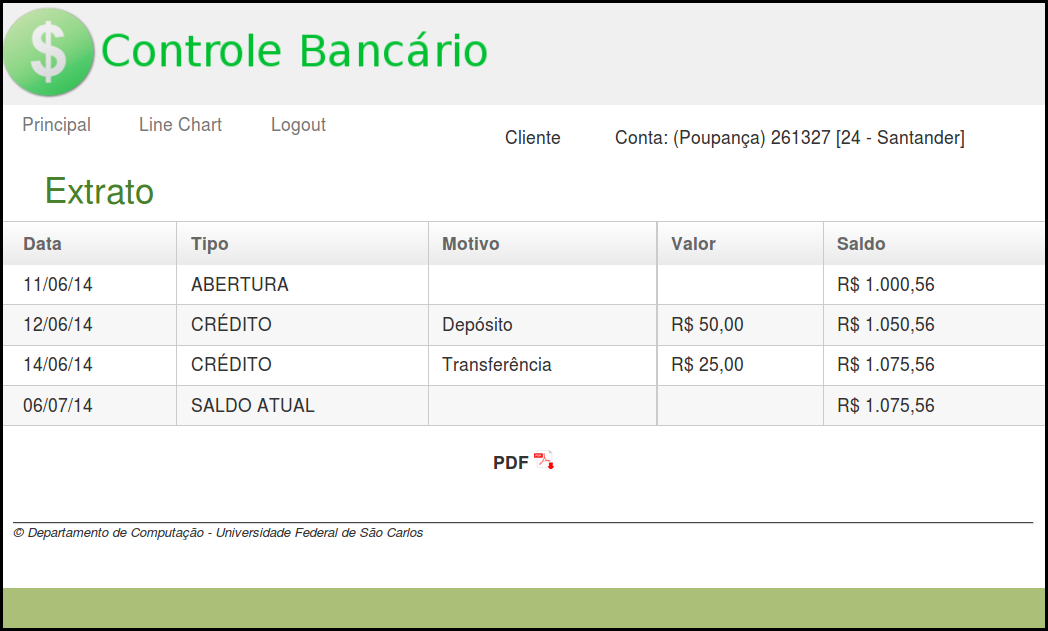
\includegraphics[width=12cm]{extrato}
\caption{Extrato Bancário em formato HTML}
\label{figExtratoHTML}
\end{figure}

Conforme   pode-se   observar,   o   {\it  template}   {\bf   extrato/\_pdf.gsp}
(Código~\ref{codPdfTemplate}) define  uma página HTML que será  convertida em um
arquivo  PDF.  Figura~\ref{figExtratoPDF}  apresenta  um exemplo  de um  extrato
bancário, em formato PDF, gerado pela ação {\bf index()}.

\begin{figure}[h]
\centering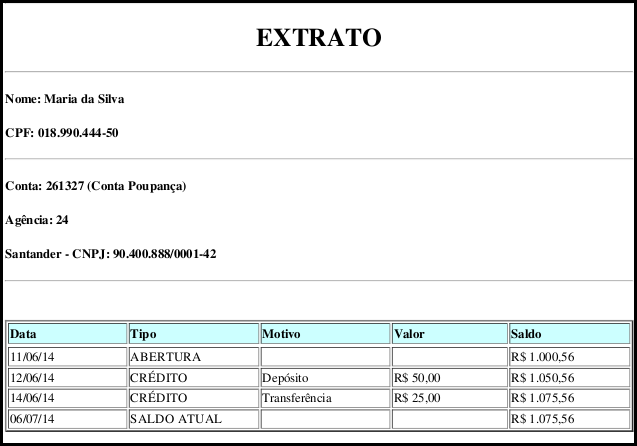
\includegraphics[width=11cm]{extratoPDF}
\caption{Extrato Bancário em formato PDF}
\label{figExtratoPDF}
\end{figure}

\newpage

\begin{lstlisting}[caption={\it Template} {\bf extrato/\_pdf.gsp}, frame=trBL,
    label=codPdfTemplate]
<%@ page import="br.ufscar.dc.dsw.ContaCorrente" %>
<%@ page import="br.ufscar.dc.dsw.ClienteFisico" %>
<hr/>
<center>
  <h1>EXTRATO</h1>
</center>
<hr/>
<h4>Nome: ${contaCliente.cliente.nome}</h4>
<h4>
  ${contaCliente.cliente instanceof ClienteFisico ? "CPF: " + contaCliente.cliente.CPF : 
                                                    "CNPJ: " + contaCliente.cliente.CNPJ}
</h4>
<hr/>
<h4>Conta: ${contaCliente.conta.numero}
  (${contaCliente.conta instanceof ContaCorrente ? "Conta Corrente" : "Conta Poupan^ç^a"})</h4>
<h4>Ag^ê^ncia: ${contaCliente.conta.agencia.numero}</h4>
<h4>${contaCliente.conta.agencia.banco} - CNPJ: ${contaCliente.conta.agencia.banco.CNPJ}</h4>
<hr/>
<br/>
<br/>
<table style="text-align: left; margin-left: auto; margin-right: auto;" class="pure-table pure-table-bordered" 
       border="2">
  <thead> 
    <tr>
      <th style="width: 200px; background-color: rgb(204, 255, 255);">Data</th>
      <th style="width: 200px; background-color: rgb(204, 255, 255);">Tipo</th>
      <th style="width: 200px; background-color: rgb(204, 255, 255);">Motivo</th>
      <th style="width: 200px; background-color: rgb(204, 255, 255);">Valor</th>
      <th style="width: 200px; background-color: rgb(204, 255, 255);">Saldo</th>
    </tr>
   </thead> 
   <tbody>
     <g:each in="${lines}" status="i" var="linha"> 
       <tr class="${(i % 2) == 0 ? 'even' : 'odd'}">
         <td><g:formatDate date="${linha.data}" type="date"/></td>
         <td>${fieldValue(bean: linha, field: "tipo")}</td>
         <td>${fieldValue(bean: linha, field: "motivo")}</td>
         <td><g:formatNumber number="${linha.valor}" type="currency"/></td>
         <td><g:formatNumber number="${linha.saldo}" type="currency"/></td>
       </tr>
     </g:each>
   </tbody>
</table>
<br/>
<br/>
<hr/>
<center>
  <h6>&copy; Departamento de Computa^çã^o - Universidade Federal de S^ã^o Carlos</h6>
  <h6><g:formatDate date="${new Date()}" type="datetime" style="LONG"/></h6>
</center>
\end{lstlisting}

A  visão  {\bf extrato/chart.gsp}  renderiza,  utilizando  o  {\it plugin}  {\bf
  google-visualization},  um gráfico  de  linhas que  representa a  movimentação
financeira  das  contas  bancárias.  A  implementação  dessa  visão  encontra-se
apresentada no Código~\ref{codChart}.  

\vspace{0.3cm}

\noindent  Conforme  pode-se  observar  essa  visão utiliza  a  {\it  tag}  {\bf
  <gvisualization:lineCoreChart>} para gerar um gráfico de linhas com os valores
({\bf columns} e {\bf lines}) retornados pela ação {\bf chart()}.  

\vspace{0.4cm}

\begin{lstlisting}[caption=Visão {\bf extrato/chart.gsp}, frame=trBL,
    label=codChart]
<%@ page import="org.grails.plugins.google.visualization.data.Cell; 
                 org.grails.plugins.google.visualization.util.DateUtil" %>
<html>
  <head>
    <title>Movimenta^çã^o Financeira</title>
    <meta name="layout" content="main" />
    <gvisualization:apiImport/>
    <r:require module="pure-all" />
  </head>
  <body>
    <div class="pure-menu pure-menu-open pure-menu-horizontal">
      <ul>
        <li><a class="home" href="${createLink(uri: '/')}"><g:message code="default.home.label"/></a></li>
        <li><g:link controller="extrato"><g:message code="extrato.statement"/></g:link></li>
        <li><g:link controller="logout">Logout</g:link></li>
      </ul>
    </div>
    <div id="list-transacao" class="content scaffold-list" role="main">
       <div id="linechart"></div>
       <gvisualization:lineCoreChart elementId="linechart" width="${800}" height="${300}" 
                      title="Movimenta^çã^o Financeira" columns="${columns}" data="${lines}" />
    </div>
  </body>
</html>
\end{lstlisting}

\newpage

\noindent   Figura~\ref{figLineChart}  apresenta  um   exemplo  de   um  gráfico
renderizado  pela ação  {\bf chart.gsp}.   Esse gráfico  ilustra  a movimentação
financeira (créditos e débitos) de uma conta bancária.

\vspace{0.3cm}

\begin{figure}[h]
\centering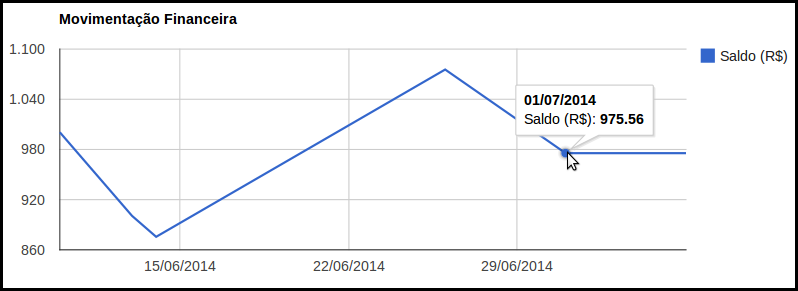
\includegraphics[width=14cm]{lineChart}
\caption{Movimentação financeira das contas bancárias}
\label{figLineChart}
\end{figure}

\section{Internacionalização - Mensagens I18n}
\index{Internacionalização~-~I18n}

\vspace{0.5cm}

Conforme pode-se observar pelas visões apresentadas/discutidas nesse capítulo, a
{\it tag} {\bf <g:message>} é utilizada para inserir rótulos internacionalizados
nessas  visões.  Dessa  forma, é  necessário adicionar  uma tradução,  para cada
idioma desejado, desses rótulos nos arquivos presentes no diretório {\bf i18n}. 

\vspace{0.2cm}

\noindent  Figura~\ref{figI18n} apresenta  a tradução  desses rótulos  que foram
inseridos  no arquivo  {\bf messages\_pt\_BR.properties}  ({\it  Message Bundle}
para o Português do Brasil).  

\vspace{0.3cm}

\begin{figure}[htbp]
\begin{mdframed}
\begin{footnotesize}
\begin{verbatim}
# Visão cliente/index.gsp
search.label=Busca de Cliente

# Visão main/index.gsp
main.options = Opções

# Visões - Controlador Transacao
transacao.main  = Conta Cliente & Caixa Eletrônico
transacao.value = Valor
transacao.data = Data
transacao.quem = Quem
transacao.motivo = Motivo
transacao.tipo = Tipo

# Visões - Controlador Extrato
extrato.statement = Extrato
extrato.chart = Line Chart
extrato.valor = Valor
extrato.saldo = Saldo
extrato.saveaspdf = PDF
\end{verbatim}
\end{footnotesize}
\end{mdframed}
\caption{Mensagens internacionalizadas}
\label{figI18n}
\end{figure}

\newpage

\section{Serviço {\it web} REST}\label{secWebREST}
\index{Serviços {\it web} REST}

\vspace{0.5cm}

REST  não é  uma tecnologia  em si,  pode ser  considerada mais  como  um padrão
arquitetural. O padrão arquitetural REST é  muito simples e envolve apenas o uso
simples de  XML ou  JSON como meio  de comunicação,  em conjunto com  padrões na
definição de  URLs que são  ``representações'' do sistema subjacente,  e métodos
HTTP, como GET, PUT,  POST e DELETE. Cada método HTTP é  mapeado para um tipo de
ação  do controlador.  Por exemplo,  o método  GET é  mapeado para  operações de
recuperação, o método  PUT é mapeado para operações de criação,  o método POST é
mapeado para operações de atualização e  assim por diante. Neste sentido REST se
encaixa muito bem com as operações CRUD. 

\vspace{0.2cm}

\noindent Essa seção  descreve a implementação de um serviço  {\it web} REST que
retorna uma lista  (em formato JSON ou XML) de agências  de um determinado banco
(parâmetro {\bf numero}). O controlador {\bf AgenciaController} é a escolha mais
óbvia para ser o responsável  por prover essa nova funcionalidade.  Dessa forma,
Código~\ref{codAgenciaController2}  apresenta  a   implementação  da  ação  {\bf
  list()},   do   controlador    {\bf   AgenciaController},   responsável   pela
implementação do serviço {\it web}  REST. Por questão de brevidade, apenas serão
apresentadas as mudanças realizadas nesse controlador.

\vspace{0.5cm}

\begin{lstlisting}[caption=Controlador  {\bf AgenciaController},  frame  = trBL,
    float=htbp, label=codAgenciaController2] 
import grails.converters.JSON
import grails.converters.XML

// Demais imports do controlador AgenciaController

class AgenciaController { 

    // Demais a^çõ^es/atributos/m^é^todos do controlador AgenciaController
   
    @Secured('IS_AUTHENTICATED_ANONYMOUSLY')
    def list() {
        
        def banco = Banco.findAllByNumero(params.numero)
        def agencias = Agencia.findAllByBanco(banco)
        def estado = Estado.findBySigla(params.estado)
        def cidade = Cidade.findByNomeAndEstado(params.cidade, estado)
        
        List<Info> lista = new ArrayList<Info>()
        
        agencias.each {
            
            if (!params.cidade || it.endereco.cidade == cidade) {
                Info info = new Info(it.banco.nome, it.numero, 
                    it.nome, it.endereco.toString())
            
                lista.add(info)
            }
        }
            
        withFormat {
            json { render lista as JSON }
            xml { render lista as XML }
        }
    }
}
\end{lstlisting}

\begin{itemize}

\vspace{0.5cm}

\item  A anotação  {\bf  @Secured('IS\_AUTHENTICATED\_ANONYMOUSLY')} indica  que
  esse serviço {\it web} é público e pode ser acessado por qualquer usuário e/ou
  aplicação.  

\vspace{0.5cm} 

\item  É importante  salientar que  a  ação {\bf  list()} retorna  uma lista  de
  instâncias  da classe  {\bf  Info}.   Conforme pode-se  observar,  a lista  de
  instâncias da classe  {\bf Info} é construída através da  iteração da lista de
  agências    associadas    a    um    determinado   banco    (parâmetro    {\bf
    numero}).   Opcionalmente,  a ação  {\bf  list()}  pode  filtrar essa  lista
  visando  apenas  retornar  as  agências  situadas em  uma  determinada  cidade
  (parâmetros {\bf cidade} e {\bf estado}); 

\vspace{0.5cm}

\item      A     classe      Java     {\bf      Info}\footnote{Arquivo:     {\bf
    src/br/ufscar/dc/dsw/Info.java}}    (Código~\ref{codInfo})    armazena    as
  informações  (atributos:  {\bf numero},  {\bf  nome},  {\bf  endereco} e  {\bf
    banco}) relacionadas às agências bancárias.  

\vspace{0.5cm}

\item Por  fim, a ação {\bf  list()} constrói a  saída ao renderizar a  lista de
  instâncias da classe {\bf Info} (em formato JSON ou XML).  A conversão para os
  formatos JSON ou XML é realizada  através da utilização das classes {\bf JSON}
  e {\bf XML} do pacote {\bf grails.converters}. 

\end{itemize}

\begin{lstlisting}[caption=Classe  Java   {\bf  Info},  frame=trBL,  float=htbp,
    label=codInfo] 
package br.ufscar.dc.dsw;

public class Info {
    
    private final int numero;

    private final String nome;

    private final String endereco;

    private final String banco;

    public Info(String banco, int numero, String nome, String endereco) {
        this.banco = banco;
        this.numero = numero;
        this.nome = nome;
        this.endereco = endereco;
    }

    public String getBanco() {
        return banco;
    }

    public String getEndereco() {
        return endereco;
    }

    public String getNome() {
        return nome;
    }

    public int getNumero() {
        return numero;
    }
    
    
}
\end{lstlisting}

Figura~\ref{figJSON} ilustra  o acesso  desse serviço {\it  web} através  da URL
{\footnotesize\url{http://localhost:8080/ControleBancarioV4/agencia/list.json?numero=1}}.
É importante salientar  que essa URL define a ação a  ser acessada: {\bf list()}
do controlador {\bf AgenciaController}.  Adicionalmente, essa URL define o valor
do parâmetro {\bf numero} e o formato da resposta (formato JSON).

\vspace{0.5cm}

\begin{figure}[h]
\centering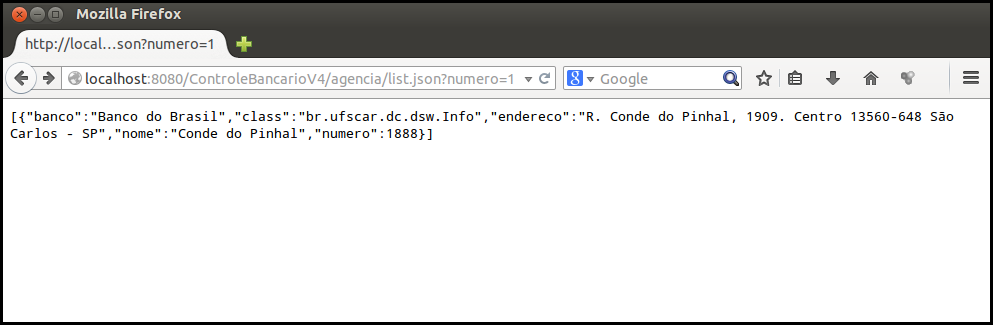
\includegraphics[width=15cm]{restJSON}
\caption{Serviço {\it web} REST: Formato JSON}
\label{figJSON}
\end{figure}

Analogamente, Figura~\ref{figXML} ilustra o acesso desse serviço {\it web} através da URL
{\footnotesize\url{http://localhost:8080/ControleBancarioV4/agencia/list.xml?numero=1}}. 
Novamente  essa URL define  a ação  a ser  acessada, o  valor do  parâmetro {\bf
  numero} e o formato da resposta (formato XML). 

\vspace{0.5cm}

\begin{figure}[h]
\centering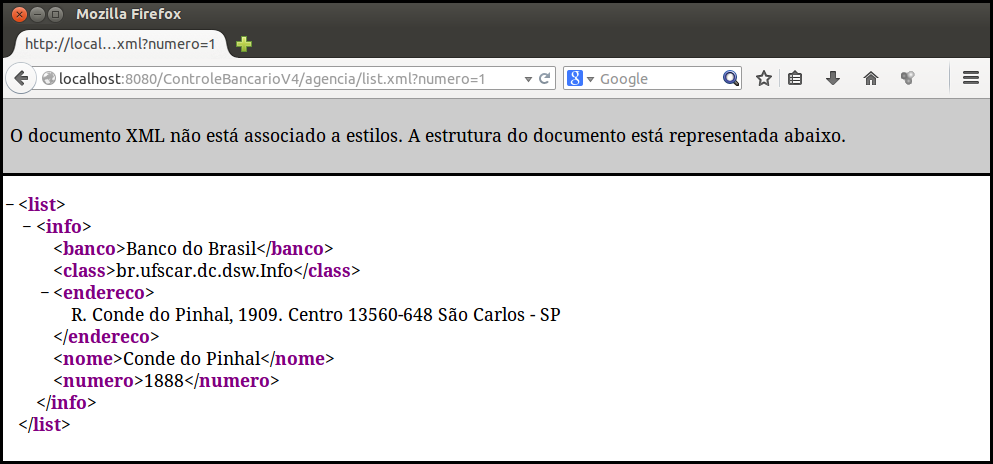
\includegraphics[width=15cm]{restXML}
\caption{Serviço {\it web} REST: Formato XML}
\label{figXML}
\end{figure}

\section{Considerações finais}

\vspace{0.3cm}


Esse  capítulo apresentou  a quarta  versão da  implementação da  aplicação {\bf
  ControleBancario}.         O        código-fonte        dessa        aplicação
({\footnotesize\texttt{ControleBancarioV4.zip}}) encontra-se  disponível no {\it
  Moodle}         do        curso,        localizado         no        endereço:
{\footnotesize\url{http://moodle.latosensu.dc.ufscar.br}}. Seguindo os passos do
tutorial   apresentado   obtem-se   esse   mesmo  código   da   aplicação   {\bf
  ControleBancario}.  


